%% Template para dissertação/tese na classe UFPEthesis
%% versão 0.9.2
%% (c) 2005 Paulo G. S. Fonseca
%% www.cin.ufpe.br/~paguso/ufpethesis

%% Carrega a classe ufpethesis
%% Opções: * Idiomas
%%           pt   - português (padrão)
%%           en   - inglês
%%         * Tipo do Texto
%%           bsc  - para monografias de graduação
%%           msc  - para dissertações de mestrado (padrão)
%%           qual - exame de qualificação doutorado
%%           prop - proposta de tese doutorado
%%           phd  - para teses de doutorado
%%         * Mídia
%%           scr  - para versão eletrônica (PDF) / consulte o guia do usuario
%%         * Estilo
%%           classic - estilo original à la TAOCP (deprecated)
%%           std     - novo estilo à la CUP (padrão)
%%         * Paginação
%%           oneside - para impressão em face única
%%           twoside - para impressão em frente e verso (padrão)
\documentclass[bsc]{ufpethesis}

%% Preâmbulo:
%% coloque aqui o seu preâmbulo LaTeX, i.e., declaração de pacotes,
%% (re)definições de macros, medidas, etc.

\usepackage{indentfirst}
\usepackage{setspace}
\usepackage{url}
\usepackage{scrextend}
\addtokomafont{labelinglabel}{\sffamily}
\usepackage{suffix}
\usepackage[withpage]{acronym} % optional command: printonlyused
\usepackage{listings}
\usepackage{color}
\usepackage{float}
\usepackage{booktabs} % pra formatar as tabelas
\usepackage{subfig} %para as subfiguras

\definecolor{dkgreen}{rgb}{0,0.6,0}
\definecolor{gray}{rgb}{0.5,0.5,0.5}
\definecolor{mauve}{rgb}{0.58,0,0.82}

\onehalfspacing

%% Identificação:

% Universidade
% e.g. \university{Universidade de Campinas}
% Na UFPE, comente a linha a seguir
%%\university{Universidade Federal de Pernambuco}

% Endereço (cidade)
% e.g. \address{Campinas}
% Na UFPE, comente a linha a seguir
%%\address{<CIDADE DA IES>}

% Instituto ou Centro Acadêmico
% e.g. \institute{Centro de Ciências Exatas e da Natureza}
% Comente se não se aplicar
\institute{Centro de Tecnologia e Geociências}

% Departamento acadêmico
% e.g. \department{Departamento de Informática}
% Comente se não se aplicar
\department{Departamento de Eletrônica e Sistemas}

% Programa de pós-graduação
% e.g. \program{Pós-graduação em Ciência da Computação}
\program{Bacharelado em Engenharia Eletrônica}

% Área de titulação
% e.g. \majorfield{Ciência da Computação}
\majorfield{Engenharia Eletrônica}

% Título da dissertação/tese
% e.g. \title{Sobre a conjectura $P=NP$}
\title{Controle e monitoramento de sinalização semafórica em vias urbanas utilizando microcontroladores}

% Data da defesa
% e.g. \date{19 de fevereiro de 2003}
\date{<DATA DA DEFESA>}

% Autor
% e.g. \author{José da Silva}
\author{Matheus da Mota Nogueira}

% Orientador(a)
% Opção: [f] - para orientador do sexo feminino
% e.g. \adviser[f]{Profa. Dra. Maria Santos}
\adviser{Gilson Jerônimo da Silva Junior}

% Orientador(a)
% Opção: [f] - para orientador do sexo feminino
% e.g. \coadviser{Prof. Dr. Pedro Pedreira}
% Comente se não se aplicar
%\coadviser{NOME DO(DA) CO-ORIENTADOR(A)}

%% Inicio do documento
\begin{document}

%%
%% Parte pré-textual
%%
\frontmatter

% Folha de rosto
% Comente para ocultar
\frontpage

% Portada (apresentação)
% Comente para ocultar
\presentationpage

% Dedicatória
% Comente para ocultar
\begin{dedicatory}
    Dedico este trabalho a todos que o tornaram possível.
\end{dedicatory}

% Agradecimentos
% Se preferir, crie um arquivo à parte e o inclua via \include{}
\acknowledgements
    Agradeço primeiramente a Deus por sua graça e luz em minha vida, aos meus pais Adelmo e Aparecida e a minha irmã Laura por todo o apoio, amor e compreensão, à minha namorada Mirla por estar sempre ao meu lado frente a todas as dificuldades, aos meus queridos amigos Paulo, Felipe, Samuel e Matheus, e ao meu orientador Prof. Gilson.

% Epígrafe
% Comente para ocultar
% e.g.
%  \begin{epigraph}[Tarde, 1919]{Olavo Bilac}
%  Última flor do Lácio, inculta e bela,\\
%  És, a um tempo, esplendor e sepultura;\\
%  Ouro nativo, que, na ganga impura,\\
%  A bruta mina entre os cascalhos vela.
%  \end{epigraph}
\begin{epigraph}{Abraham Lincoln}
Não sou obrigado a vencer, mas tenho o dever de ser verdadeiro. Não sou obrigado a ter sucesso, mas tenho o dever de corresponder à luz que tenho.
\end{epigraph}

% Resumo em Português
% Se preferir, crie um arquivo à parte e o inclua via \include{}
\resumo
A iluminação de LED apresenta algumas vantagens diante das tradicionais iluminações fluorescentes e incandescentes. Lâmpadas ou fitas de LED são em geral mais eficientes, compactas e oferecem vantagens como variedade de cores em comparação às variantes tradicionais de iluminação e por isso vêm sendo utilizadas tanto em iluminação pública como em decoração e em pequenos dispositivos. A facilidade de controlar sua intensidade por meio do rápido chaveamento de sua potência é outro atrativo, principalmente quando se trata do uso de microcontroladores conectados à internet. Este trabalho apresenta uma implementação de um sistema de iluminação com fita de LEDs brancos controlada pelo sistema embarcado "ESP-8266" por meio da troca de dados pela internet com um aplicativo móvel por meio do protocolo de internet "MQTT" com a capacidade de ligar, desligar, arbitrar a intensidade da fita no modo manual ou ter a intensidade controlada automaticamente. Serão feitas medições do consumo do sistema para demonstrar a capacidade de economia de energia do sistema proposto.

% Palavras-chave do resumo em Português
\begin{keywords}
    Iluminação, LED, MQTT, ESP8266
\end{keywords}

% Resumo em Inglês
% Se preferir, crie um arquivo à parte e o inclua via \include{}
\abstract
Led illumination holds some advantages on fluorescent and incandescent forms of illumination. LED lamps or strips are, in general more efficient, compact and have features like color variety when compared to those other forms of illumination and that's why they are utilized on public lighting, decoration or on small gadgets. Ease of controlling its intensity by fastly keying its power source is an important feature when it comes to the use of microcontrollers like those connected to the internet. This work demonstrates an implementation of a lighting system with a white LED strip controlled by the embedded system "ESP-8266"  by means of data exchange on the internet with a mobile application with the MQTT internet protocol and it has the capability of turning on, off, setting the led strip's intensity or even setting the automatic intensity mode. Measurements will be taken in order to demonstrate the energy saving capability of this proposed system. 
% Palavras-chave do resumo em Inglês
\begin{keywords}
    Illumination, LED, MQTT, ESP8266
\end{keywords}

% Sumário
% Comente para ocultar
\tableofcontents

% Lista de figuras
% Comente para ocultar
\listoffigures

% Lista de tabelas
% Comente para ocultar
\listoftables

\chapter*{Lista de Siglas}
\begin{acronym}[MQTT]
    \acro{LED}{\textit{Light Emitting Diode}}
    \acro{RAM}{\textit{Random-Access Memory}}
    \acro{ROM}{\textit{Read-Only Memory}}
    \acro{ULA}{Unidade Lógica e Aritmética}
    \acro{UC}{Unidade de Controle}
    \acro{MIPS}{\textit{Million Instructions Per Second}}
    \acro{I/O}{\textit{Input/Output}}
    \acro{EPROM}{\textit{Erasable Programmable Read-Only Memory}}
    \acro{EEPROM}{\textit{Electrically Erasable Programmable Read-Only Memory}}
    \acro{ADC}{\textit{Analog-to-Digital Converter}}
    \acro{DAC}{\textit{Digital-to-Analog Converter}}
    \acro{RX}{\textit{Receiver}}
    \acro{TX}{\textit{Transmitter}}
    \acro{USART}{\textit{Universal Synchronous and Asynchronous Receiver-Transmitter}}
    \acro{USB}{\textit{Universal Serial Bus}}
    \acro{TBJ}{Transistor Bipolar de Junção}
    \acro{TRIAC}{\textit{Triode for Alternating Current}}
    \acro{CPU}{\textit{Central Processing Unit}}
\end{acronym}

%%
%% Parte textual
%%
\mainmatter

% É aconselhável criar cada capítulo em um arquivo à parte, digamos
% "capitulo1.tex", "capitulo2.tex", ... "capituloN.tex" e depois
% incluí-los:
\chapter{Introdução}

Qualquer pessoa, que necessite se deslocar pela cidade, tem contato com o trânsito em vias urbanas e tem sua rotina influenciada pelo mesmo, seja dirigindo um carro, andando de ônibus ou atravessando ruas. O conceito de trânsito pode ser aplicado tanto para pedestres como para motoristas (e passageiros), pois ele representa a utilização das vias por pessoas, veículos e animais, isolados ou em grupos, conduzidos ou não, para fins de circulação, parada, estacionamento e operação de carga ou descarga \cite{lei}.
%[http://www.planalto.gov.br/ccivil_03/LEIS/L9503.htm]

Com essa definição, é evidente que as vias urbanas são um espaço compartilhado entre diversos automóveis e pedestres, de modo que é necessário estar atento a dois parâmetros: segurança e redução de riscos, e controle e gerenciamento do fluxo das vias.

A questão da segurança é importante pois o trânsito seguro é um direito de todos e um dever dos órgãos e entidades do Sistema Nacional de Trânsito \cite{manual3}, %[Manual de direção defensiva DENATRAN]
e sem devido controle e sinalização de vias, existe um aumento considerável de riscos de acidentes em locais de conflito entre movimentos de veículos, em locais de cruzamento de vias, ou entre veículos e pedestres, em locais de travessia.

O controle de fluxo é importante, pois com o aumento constante das frotas de veículos nos centros urbanos, a tendência é a sobrecarga da capacidade das vias mais movimentadas. A capacidade de uma via pode ser descrita como o fluxo máximo de veículos permitidos, sem que haja atrasos significativos nos tempos de viagens. Uma sobrecarga na capacidade de uma via resulta em congestionamentos, que trazem pontos negativos ao dia a dia das pessoas envolvidas, como exposição a potenciais perigos urbanos, aumento indesejável do tempo de viagem e aumento de estresse.

Por questões de limitações de espaço urbano, não é possível a expansão indefinida da largura das vias, para comportar mais veículos, por isso, para evitar, ou reduzir, o congestionamento, é necessária a utilização de sinalização e equipamentos eficientes e tecnológicos, com o intuito de realizar algum tipo de controle, a fim de garantir a segurança de todos e a organização dos fluxos, assim como a redução de riscos de acidentes.

\section{Motivação}

O Brasil possui 97 milhões de veículos, dos quais 5.4 milhões chegaram às ruas no ano de 2017, desse número quase 90\% é composto por veículos que circulam diariamente em vias urbanas, como automóveis, motocicletas e ônibus. Essa quantidade vem crescendo a cada ano, com uma média de 3.84 milhões de novos veículos por ano, nos últimos cinco anos. %[http://www.denatran.gov.br/index.php/estatistica/610-frota-2017]. 
Uma grande quantidade de veículos em circulação pode facilmente sobrecarregar a capacidade das vias urbanas, trazendo consequências para o trânsito.

Pesquisas realizadas no começo do ano de 2018 mostraram que, em horários de pico, o trânsito nas principais capitais brasileiras pode resultar em tempos de viagens até 77\% mais demorados que o usual\cite{recife}, %[http://jc.ne10.uol.com.br/blogs/deolhonotransito/2018/03/27/recife-capital-com-o-transito-mais-lento-do-pais-de-novo/]
isso é uma consequência da quantidade de veículos nas ruas. Além disso, existem pesquisas relacionando o trânsito como um gerador de estresse na população, principalmente nos em condutores veiculares, e o estresse como uma das principais causas das agressividades no trânsito \cite{stress}\cite{stress2}.  %[https://www.researchgate.net/profile/Vinicius_Ferreira3/publication/237480019_Comportamentos_no_transito_e_causas_da_agressividade/links/02e7e528bc018b2f72000000/Comportamentos-no-transito-e-causas-da-agressividade.pdf] [https://singep.org.br/6singep/resultado/406.pdf] [http://www2.fm.usp.br/gdc/docs/iof_89_estressetrans.pdf].

Com o intuito de reduzir riscos e aumentar a organização das vias, é utilizada a sinalização de trânsito. A sinalização de trânsito é o elemento de ligação entre o técnico, o usuário da via, motoristas e pedestres e os agentes de fiscalização. Seu objetivo principal é o de garantir a utilização adequada da via, no sentido da segurança e fluidez do tráfego como um todo. Para atingir este objetivo, é necessário que a sinalização contenha uma mensagem clara e inconfundível e que seja plenamente visível. Desse modo, iniciou-se a padronização dos elementos responsáveis por realizar a sinalização, em cores, formatos, dimensões e critérios de utilização\cite{CET}. %[http://www.cetsp.com.br/media/391986/msuvol01_introducaorev01.pdf]. 
O foco deste trabalho é a sinalização semafórica das vias urbanas.

\begin{figure}[ht]
    \begin{center}
    \subfloat[Semáforo veicular]{\label{veicular}
    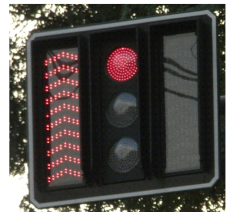
\includegraphics{figuras/semaforo.PNG}}
    \subfloat[Semáforo de pedestres]{\label{pedestre}
    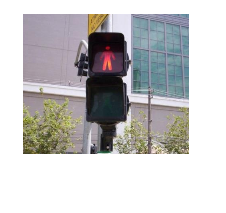
\includegraphics{figuras/semaforo_ped.PNG}}
    \caption[Semáforos]{Exemplos de sinalização semafórica.}
    \end{center}
    \label{semaforos}
\end{figure}
%http://www.cetsp.com.br/media/517462/nt252.pdf (semaforo veicular CET)(a)
%http://www.cetsp.com.br/media/478292/nt241.pdf (foco pedestres)(b)

A Figura 1.1 apresenta exemplos de sinalização semafórica, utilizados no controle de fluxos veicular (\ref{veicular}) e de pedestres (\ref{pedestre}).

Além de apresentar um sistema que realiza o controle de sinalização semafórica de maneira automatizada, também serão expostos resultados de simulações realizadas, com o intuito de demonstrar o impacto do sistema em cruzamentos de vias urbanas.

\section{Objetivo}

O objetivo desse trabalho é apresentar produtos que têm como finalidade solucionar os problemas apresentados na introdução ao assunto: gerenciamento e controle da segurança e do fluxo de veículos e pedestres nas vias urbanas. A solução apresentada é um conjunto de sistemas, com objetivos específicos cada, que, integrados, são capazes de realizar as atividades desejadas de controle de sinalização semafórica.

Além disso, serão apresentadas simulações realizadas, sob diferentes configurações do sistema, de modo a demonstrar os diferentes meios de abordagem para solucionar o problema de organização de sinalização semafórica.


\section{Estrutura do trabalho}

Esse trabalho é composto por 5 capítulos, sendo este o primeiro, e os 4 restantes são descritos, brevemente, a seguir:

\begin{itemize}
    \item Capítulo 2 - Nesse capítulo são descritas as tecnologias e fundamentações teóricas das soluções propostas
    \item Capítulo 3 - Nesse capítulo são descritos os detalhes dos sistemas implementados e como ocorre a integração entre eles
    \item Capítulo 4 - Nesse capítulo é apresentado o software utilizado para realizar as simulações e os cenários simulados
    \item Capítulo 5 - Nesse capítulo são analisados os dados obtidos das simulações
\end{itemize}

\chapter{Fundamentação Teórica}

A sinalização semafórica pode ser feita com uma de duas funções planejadas: a de regulamentar o direito de passagem de fluxos de veículos e pedestres nas vias, ou de advertir os condutores de veículos e pedestres sobre obstáculos ou situações perigosas nas vias. A composição da sinalização semafórica é um conjunto de indicações luminosas, acionadas alternadamente ou intermitentemente, fixado em posições, próximas à via, que as tornem fáceis de identificar e interpretar para condutores e pedestres\cite{sinalizacao}. 
%[http://meusite.mackenzie.br/professor_cucci/ManualSemaforos2014.pdf]

A tabela \ref{tab: focos} mostra as definições de formas e dimensões da sinalização semafórica a ser utilizada, dependendo de sua finalidade.

\begin{table}[H]
\centering
\caption{Definições de formas e dimensões}
\label{tab: focos}
\begin{tabular}{@{}lllll@{}}
\toprule
Semáforos destinados a & Forma do foco & Dimensão da lente (mm) \\ \midrule
Veículos automotores & Circular & Diâmetro de 200 ou 300 \\
Bicicletas & Circular & Diâmetro de 200 ou 300 \\
Faixas reversíveis          &	Quadrada & Lado de 300		  \\
Advertência & Circular & Diâmetro de 200 ou 300 \\
Pedestres & Quadrada & Lado de 200 ou 300 \\
\bottomrule
\end{tabular}
\end{table}
% http://meusite.mackenzie.br/professor_cucci/ManualSemaforos2014.pdf

A maneira mais eficiente de realizar o controle de sinalização semafórica, controlando e temporizando o acendimento alternado das indicações luminosas é dada utilizando circuitos eletrônicos, feitos especificamente para essa finalidade. A esse sistema dá-se o nome de sistema embarcado. 

\section{Sistemas embarcados}

Um sistema embarcado pode ser entendido como uma combinação de \textit{hardware} (placas de circuito impresso, circuitos integrados, componentes eletrônicos) e \textit{software} (programação carregada em processadores), que é feito para um fim específico e pré-determinado, sendo assim bastante confiável e otimizado, e possibilitando menor custo nos projetos (um sistema feito para funções generalizadas costuma custar mais caro). A interação com o ambiente externo se dá por meio de sensores e atuadores, apresentando uma interface simplificada, dependendo da utilização, como botões de \textit{on/off} e \ac{LED} de sinalização\cite{book4}. 
%[Michael Barr. Programming Embedded Systems in C and C++. cap1]

\begin{figure}[ht]
    \begin{center}
    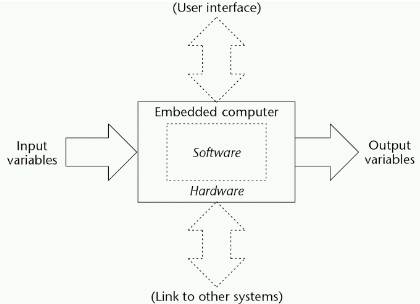
\includegraphics{figuras/embedded.PNG}
    \end{center}
    \caption[]{Visão geral da integração de um sistema embarcado}
    \label{embarcado}
\end{figure}
%[http://www.eletrica.ufpr.br/mehl/te200/aulas/embarcados.pdf]

O avanço da tecnologia, porém, permitiu a confecção de sistemas cada vez mais elaborados e capazes, fazendo com que os sistemas embarcados se tornem cada vez mais abrangentes, contradizendo a definição de sistema feito para fins específicos. Para utilização de sistemas embarcados em seus projetos, um projetista deve estudar os requisitos de tal projeto, escolher o \textit{hardware} específico para a realização das tarefas e, por fim, escrever um \textit{software} otimizado para o circuito montado\cite{embedded}. %[http://www.eletrica.ufpr.br/mehl/te200/aulas/embarcados.pdf].

Sistemas embarcados podem ser encontrados em diversos dispositivos do dia a dia, realizando diferentes tipos de controle, e em alguns casos, agindo em conjunto com outros sistemas embarcados, compondo um sistema maior e completo.
Um sistema embarcado necessita de um núcleo de processamento para realizar as tarefas necessárias, chamado de processador. Além disso, necessita também de circuitos periféricos que permitam que o processador se comunique com o meio externo. Dá-se o nome de microcontrolador, ao conjunto de um processador com tais periféricos, em um único \textit{chip}.
O foco deste trabalho é falar sobre a utilização de microcontroladores como solução para controle de sinalização semafórica. 

\subsection{Microprocessadores}

Os processadores são a unidade central de um sistema embarcado que processa dados e instruções, eles realizam as tarefas e controlam o funcionamento dos periféricos, funcionam com um \textit{clock}, recebem dados binários como entrada, armazenando-os em registradores, e realizam operações com tais dados, enviando o resultado como saída\cite{book3}. 
%[Osborne, Adam (1980). An Introduction to Microcomputers. Volume 1: Basic Concepts (2nd ed.). Berkeley, California: Osborne-McGraw Hill.]

\begin{figure}[ht]
    \begin{center}
    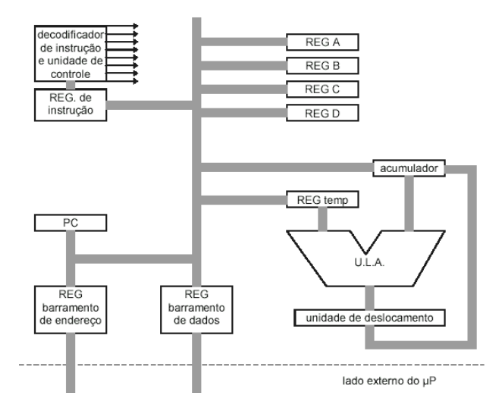
\includegraphics{figuras/processor.PNG}
    \end{center}
    \caption[Sistema embarcado]{Visão geral da integração de um sistema embarcado.}
    \label{processor}
\end{figure}

%[http://iris.sel.eesc.usp.br/sel433a/Micros.pdf]

A Figura \ref{processor} apresenta de modo simplificado a estrutura interna de um microprocessador, onde pode-se notar os registradores, que são armazenadores de dados, e suas duas unidades básicas: a \ac{ULA}, onde ocorrem as operações lógicas e aritméticas, e a \ac{UC}, responsável pela execução das instruções. %http://iris.sel.eesc.usp.br/sel433a/Micros.pdf
Os processadores possuem parâmetros que definem o modo e a velocidade de operação dos mesmos, que serão explicados a seguir.

\subsubsection{Capacidade de processamento}

A capacidade de processamento, com a qual um processador consegue trabalhar, representa o número de \textit{bits} que pode ser processado por instrução, também chamado de palavra. Uma instrução é definida como uma única ação que o processador pode executar por vez %http://iris.sel.eesc.usp.br/sel433a/Micros.pdf 
Um processador com capacidade de processamento de 4 \textit{bits}, por exemplo, consegue processar dados de até 4 \textit{bits} (equivalente a \(2^4\), ou 16) por vez. Com o avanço da tecnologia, a capacidade dos processadores foi aumentando drasticamente, sendo encontrados, hoje, nos microcontroladores no mercado, dispositivos com capacidades que variam entre 8, 16 e 32 \textit{bits} (\(2^8\) = 256; \(2^16\) = 65536; \(2^32\) = 4294967296).

\subsubsection{Velocidade de \textit{Clock}}

Frequência do \textit{clock}. Quantidade de ciclos por segundo. Além disso, existe a quantidade de instruções por segundo. A velocidade do \textit{clock} de um processador determina o quão rápido ele consegue realizar as suas instruções. O intel 4004 possuía um \textit{clock} máximo de 740 kHz, que equivale a 740 mil pulsos por segundo. Os microprocessadores atuais alcançam velocidades acima de 500 Mhz (mais de 650 vezes mais rápidos). 

Além da velocidade de \textit{clock}, os processadores possuem um parâmetro que determina quantos ciclos desse \textit{clock} são necessários para que uma instrução seja realizada. O Intel 4004 necessitava de 8 ciclos por instrução, enquanto alguns microprocessadores modernos conseguem realizar 945 \ac{MIPS} com um \textit{clock} de 600 MHz (resultando em mais de 1.5 instruções por ciclo de \textit{clock})\cite{clock}. %[http://ww1.microchip.com/downloads/en/DeviceDoc/60001525A.pdf]

\begin{figure}[ht]
    \begin{center}
    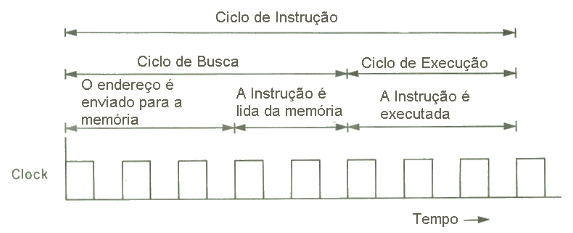
\includegraphics{figuras/clock.PNG}
    \end{center}
    \caption[Sequencia de instrução]{Processo de execução de instrução do processador.}
    \label{clock}
\end{figure}

A Figura \ref{clock} mostra o comportamento do sinal de \textit{clock}, e as atividades realizadas, durante o mesmo, pelo microprocessador para realizar uma instrução.

\subsubsection{Periféricos}

Mesmo sendo o núcleo computacional do sistema, um microprocessador não seria de grande utilidade, sem a integração com elementos externos, como memórias, para armazenamento de dados, e canais de entrada e saída de dados (\ac{I/O}). A maneira mais simplificada de integrar os periféricos ao microprocessador, como foi integrado o Intel 4004, é utilizando uma memória \ac{RAM}, uma memória \ac{ROM} e um canal de portas \ac{I/O} (no caso do 4004, era um canal de 4 \textit{bits}).

\begin{figure}[ht]
    \begin{center}
    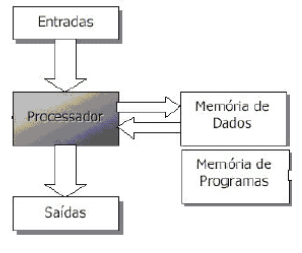
\includegraphics{figuras/processor_periph.PNG}
    \end{center}
    \caption[Periféricos do processador]{Interação do processador com as memórias.}
    \label{perifericos}
\end{figure}

%http://iris.sel.eesc.usp.br/sel433a/Micros.pdf

%\begin{labeling}{17.5.3.3}
%    \item[17.5.3] Em todos os locais de trabalho deve haver iluminação adequada, natural ou artificial, geral ou suplementar, apropriada à natureza da atividade.
%    \item[17.5.3.1]  A iluminação geral deve ser uniformemente distribuída e difusa.
%   \item[17.5.3.2] A iluminação geral ou suplementar deve ser projetada e instalada de forma a evitar ofuscamento, reflexos incômodos, sombras e contrastes excessivos.
%    \item[17.5.3.3] Os níveis mínimos de iluminamento a serem observados nos locais de trabalho são os valores de iluminâncias estabelecidos na NBR 5413, norma brasileira registrada no INMETRO.
%\end{labeling}

A memória \ac{RAM} é utilizada pelo microprocessador para armazenar e ler dados. Por se tratar de uma memória volátil, os dados contidos nela são apagados quando é desenergizada.
Já a memória \ac{ROM} é utilizada para armazenar as instruções a serem executadas pelo microprocessador. Por se tratar de uma memória não volátil, os dados salvos nela não são apagados quando o sistema é desenergizado, garantindo que o programa gravado seja sempre executado ao ligar o microprocessador. Apesar do nome, existem variantes dessa memória que permitem a regravação de dados (\ac{EPROM}, \ac{EEPROM}).

Com as memórias, o microprocessador pode executar instruções salvar dados, porém ainda é necessário um canal de comunicação com o meio externo, que é satisfeito com a integração de um canal de comunicação \ac{I/O} de dados digitais. Nos barramentos \ac{I/O}, cada entrada, ou saída, representa um \textit{bit}. 

Com esses periféricos, o microprocessador é capaz de identificar instruções, aceitar e armazenar dados vindo do ambiente externo, processar tais dados e enviar o resultado de volta ao ambiente externo. Outros periféricos podem ser integrados, e são utilizados em microprocessadores modernos. Alguns serão explicados em outras seções desse trabalho.


\subsection{Microcontroladores}

Enquanto um microprocessador é feito para realizar tarefas genéricas, ele pode ser integrado com determinados elementos periféricos, para especificar uma finalidade de uso. Quando essa combinação de dispositivos é disposta em um único chip, dá-se o nome de microcontrolador.

Um microcontrolador, de maneira simplificada, é composto de um processador, em conjunto com memórias \ac{RAM} e \ac{ROM} e um canal \ac{I/O}, tendo outras funcionalidades, dependendo da família de produtos escolhida. Um microcontrolador é um \textit{hardware} bastante versátil, podendo ser utilizado em várias aplicações que necessitem de soluções inteligentes de baixo custo, que compõe a parte do \textit{hardware} envolvido no sistema embarcado. Apesar da versatilidade, quando um microcontrolador é escolhido para um projeto, suas funções passam a ser bastante específicas, por conta do circuito eletrônico que é montado em volta dele, e do \textit{software} que é escrito especificamente para aquela finalidade.

\begin{figure}[ht]
    \begin{center}
    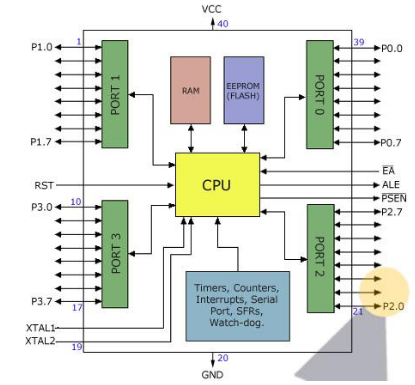
\includegraphics{figuras/microprocessador.PNG}
    \end{center}
    \caption[Microcontrolador]{Integração do processador com periféricos.}
    \label{microcontrolador}
\end{figure}
%https://elprojects.blogspot.com/2010/06/microcontroller-at89s52-description.html

A Figura \ref{microcontrolador} mostra o esquema de um microcontrolador, com um microprocessador integrado com memórias \ac{RAM} e \ac{ROM}, 4 portas de comunicação \ac{I/O} e outros periféricos.

O mercado de microcontroladores tem suas origens em 1974, com o TMS1000, apresentado como uma “calculadora em um \textit{chip}”, pela Texas Instruments. Esse dispositivo possuía uma capacidade de processamento de 4 \textit{bits}, velocidade de \textit{clock} de 400 KHz e execução de uma instrução a cada 6 ciclos de \textit{clock}, enquanto dispositivos modernos ultrapassam os 250 MHZ de velocidade e capacidade para realizar 330 milhões de instruções por segundo (1.3 instruções realizadas por ciclo de \textit{clock}), representando um aumento de mais de 600 vezes na velocidade de processamento.

Além dos periféricos já mencionados, os microcontroladores mais modernos apresentam uma vasta gama de utilidades, como conversores de sinal analógico, portas prontas para a utilização de protocolos de comunicação, módulos \textit{bluetooth}, \ac{USB}, wifi. Os periféricos mais relevantes para o escopo do trabalho serão explicados neste capítulo.

\subsubsection{Conversor de sinal analógico}

O armazenamento e processamento de um microcontrolador acontecem com a utilização de dados digitais, compostos de \textit{bits}, cujos valores só podem ser 0 ou 1. Em determinados projetos, porém, surge a necessidade de realizar a análise de um sinal analógico, como o sinal de um sensor de luminosidade, sensor de temperatura, realizar a leitura de uma lâmpada, são exemplos de sinais analógicos a serem recebidos pelo microcontrolador.

Para essa tarefa existe um periférico, integrado ao microcontrolador, que recebe o sinal analógico, e realiza a conversão para um sinal digital. Esse periférico é chamado de \ac{ADC}. A conversão A/D é realizada por meio de comparação entre o valor recebido e um valor de referência, que deve ser aplicado ao microcontrolador. Esse processo possui precisão variável, dependendo da quantidade de \textit{bits} utilizados pelo dispositivo, onde cada \textit{bit} representa uma subdivisão do valor de referência. Assim, para um valor de referência de 5 \textit{volts}, por exemplo, um \ac{ADC} de 8 \textit{bits} possui resolução de 20 mV, por meio da equação \ref{eq:teoria_1}, que representa o cálculo da resolução do \ac{ADC}.

\begin{equation}
\label{eq:teoria_1}
R = \frac{V_{ref}}{2^n}
\end{equation}

O processo oposto também é possível, em que o dispositivo converte um sinal digital em um sinal analógico (\ac{DAC}), e alguns microcontroladores já possuem essa função integrada. O funcionamento é semelhante ao do \ac{ADC}, em que é necessária a utilização de uma voltagem de referência \(V_{ref}\), e a resolução do processo é determinada pela quantidade de \textit{bits} utilizada. Um \ac{DAC} com 8 \textit{bits} tem capacidade de geração de sinal de saída com \( 2^8 \), ou \(256\) níveis de tensão distintos.

\subsubsection{Porta serial}

A porta serial, de um microcontrolador, é um canal de comunicação que utiliza dois de seus pinos para tal. Um pino funciona como receptor de mensagens (\ac{RX}), enquanto o outro envia as mensagens (\ac{TX}). A comunicação serial é dada com o envio de 1 \textit{bit} por vez, com a velocidade determinada pelo \textit{baud rate} (taxa de envio de bits), que deve ser a mesma entre os dispositivos envolvidos na comunicação.

A comunicação serial pode ser dada de forma síncrona ou assíncrona, que determina a forma de envio e recebimento de \textit{bits}. Na comunicação síncrona, a mensagem é enviada, juntamente com um \textit{clock}, e cada \textit{bit} é transmitido apenas nos momentos positivos ou negativos desse \textit{clock} (dependendo da configuração da comunicação).

\begin{figure}[ht]
    \begin{center}
    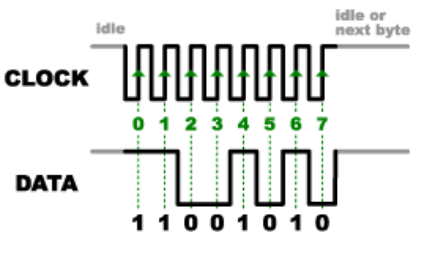
\includegraphics{figuras/sincrono.PNG}
    \end{center}
    \caption[Comunicação síncrona]{Envio de mensagem na comunicação síncrona.}
    \label{sincrono}
\end{figure}
%http://www.engineering.union.edu/~hodgsond/MER421/Winter%202015/Lectures/MER421Serial.pdf

Já na comunicação assíncrona, cada \textit{bit} é enviado independentemente, respeitando o \textit{baud rate} configurado, e recebido nessa mesma velocidade. Por não haver sincronismo no envio de informação, são enviados \textit{bits} extras, a cada mensagem transmitida, como indicação de início de transmissão, fim de transmissão e, em alguns casos, um \textit{bit} de paridade, usado para verificar a precisão da mensagem enviada.

\begin{figure}[ht]
    \begin{center}
    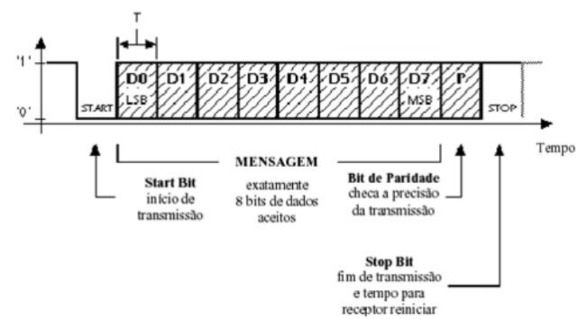
\includegraphics{figuras/assincrono.PNG}
    \end{center}
    \caption[Comunicação assíncrona]{Envio de mensagem na comunicação assíncrona.}
    \label{assincrono}
\end{figure}
%José Wilson Lima Nerys. MICROPROCESSADORES E MICROCONTROLADORES - PARTE 2 MICROCONTROLADOR 8051. 2018. 151 slides. Disponível em http://www.emc.ufg.br/~jwilson/pdf/2_Micro_Parte_2_(8051).pdf

Os microcontroladores modernos possuem capacidade de comunicação serial configurável, através da \ac{USART}, podendo assim realizar tanto a comunicação síncrona, como a assíncrona.

\subsubsection{Interrupções}

Evento que causa a suspensão temporária das atividades do microcontrolador, para que sejam realizadas rotinas específicas, de acordo com o tipo de interrupção. Após a realização da rotina de interrupção, o microcontrolador retorna ao ponto do programa em que se encontrava antes do evento. O evento causador da interrupção pode ser um fator interno ou externo\cite{8051}. %https://docente.ifsc.edu.br/rafael.grebogi/MaterialDidatico/Mecatronica/Microcontroladores/ebook%20-%20microcontrolador%208051-%20detalhado.pdf

Existem diferentes tipos de eventos que podem causar uma interrupção em um microcontrolador, e cabe ao programador definir a ordem de prioridade entre elas:
\begin{itemize}
\item \textit{Timer} - Os \textit{Timers} são contadores, de 8 ou 16 \textit{bits}, que incrementam a contagem de acordo com a frequência do oscilador utilizado, e geram uma interrupção no sistema ao ocorrer \textit{overflow} na contagem. Os \textit{Timers} podem ser configurados para contar diferentes tempos, e são normalmente utilizados como temporizadores.
\item \ac{ADC} - Uma das funcionalidades da conversão A/D de microcontroladores, é a possibilidade de configurar uma interrupção do sistema quando a conversão é finalizada.
\item Comunicação serial - Dois tipos de interrupção podem ser configuradas na comunicação serial, no envio e no recebimento da mensagem. No envio, a interrupção ocorre quando o microcontrolador detecta que o \textit{buffer} de envio se torna vazio. Já no recebimento, a interrupção ocorre assim que é detectado o recebimento de um \textit{byte}.
\item Sinais externos - Além das interrupções apresentadas, é possível, ainda, configurar determinados pinos do microcontrolador para gerarem uma interrupção do sistema, ao receber um sinal.
\end{itemize}

\section{Programação}

Para alcançar as funcionalidades desejadas do microcontrolador, é necessário que o projetista desenvolva um programa (\textit{software}) e carregue-o na memória do microcontrolador. Quando um \textit{software} é feito para um fim específico, carregado em um circuito com um objetivo claro, dá-se o nome de \textit{Firmware}. Um \textit{firmware} é um código escrito com o intuito de ser gravado apenas uma vez no \textit{hardware}, com raras modificações, normalmente em casos de correções de erros.

Cada família de microcontroladores possui um conjunto de instruções específicas a ser utilizado na sua programação. Essas instruções são escritas em \textit{Assembly}, que é uma linguagem de programação que possibilita a integração das instruções do microcontrolador com funções legíveis por humanos.

Programar em \textit{assembly}, porém, requer que o programador aprenda um novo conjunto de instruções para cada dispositivo diferente a ser utilizado. Para resolver esse problema, foram criados compiladores que permitem a utilização da linguagem C para a programação de microcontroladores, o que padroniza esse processo e proporciona facilidade no desenvolvimento de projetos com dispositivos distintos.

\section{Sistema adaptativo}

%https://www.civil.iitb.ac.in/tvm/nptel/tselnw61.pdf
%https://sci-hub.tw/https://ieeexplore.ieee.org/document/69966
%https://sci-hub.tw/https://ieeexplore.ieee.org/document/1622746
%https://sci-hub.tw/https://www.sciencedirect.com/science/article/pii/S0968090X00000474?via%3Dihub
%https://civil808.com/sites/default/files/field/files/node_3951-roger_roess_elena_prassas_william_mcshane_trafbookzz.org_.pdf
Para lidar com variações temporárias e imprevisíveis do trânsito, é necessária uma abordagem diferente da programação em tempos fixos dos semáforos. Para isso, são utilizados métodos adaptativos de controle de trânsito.
Os sistemas adaptativos são métodos para monitorar e modificar o comportamento dos semáforos, em tempo real, com o intuito de responder a variações de condições do trânsito\cite{adaptive}. Para alcançar esse objetivo, o controlador semafórico utiliza dados coletados das vias, de detectores veiculares, para otimizar os tempos de abertura dos semáforos.
O intuito de implementar um sistema adaptativo, em tempo real, é reduzir trânsito, consumo de combustível, acidentes, poluição e tempo de viagem.
Dois exemplos de sistemas, mundialmente conhecidos, que realizam o controle adaptativo de semáforo, são o SCOOT e o SCAT\cite{areacontrol}.

O SCOOT é um sistema de controle de tráfego urbano, desenvolvido pelo \textit{Transport Research Laboratory}(TRL), no Reino Unido. Seu principal objetivo é minimizar os tempos de fila na área atuante, respondendo automaticamente, em tempo real, às variações causadas no trânsito. O sistema aumenta, ou diminui, os tempos de abertura dos semáforos, de acordo com a situação momentânea do trânsito, com o intuito de minimizar o Índice de Performance (\textit{Performance Index}, ou PI), que é uma medida composta pelo atraso do percurso, comprimento de filas de veículos e paradas nas vias. Para conseguir alcançar os objetivos, o sistema conta com detectores veiculares, instalados nas vias, em locais próximos ao cruzamento em que se encontra o semáforo\cite{scoot}.

O SCAT (\textit{Sydney Co-ordinated Adaptive Traffic Control}) é outro sistema adaptativo de controle de trânsito, desenvolvido pela \textit{Roads and Traffic Authority}(RTA), na Austrália, nos anos 70. Assim como o SCOOT, o SCAT utiliza detectores veiculares, localizados nas vias, para adquirir dados referentes às condições de tráfego e realizar, em tempo real, a alteração dos tempos de abertura dos semáforos\cite{scat}.
A diferença entre os sistemas é que, enquanto o SCOOT utiliza os dados dos detectores para tentar otimizar o fluxo veicular para os ciclos futuros, o SCAT age realizando a correção dos tempos, de acordo com o ciclo anterior.



%\chapter{Materiais e Ferramentas}

A descrição dos elementos físicos usados no projeto da lâmpada inteligente pode ser resumida pelo esquema geral do projeto na Figura \ref{esquema}.

\begin{figure}[ht]
    \begin{center}
    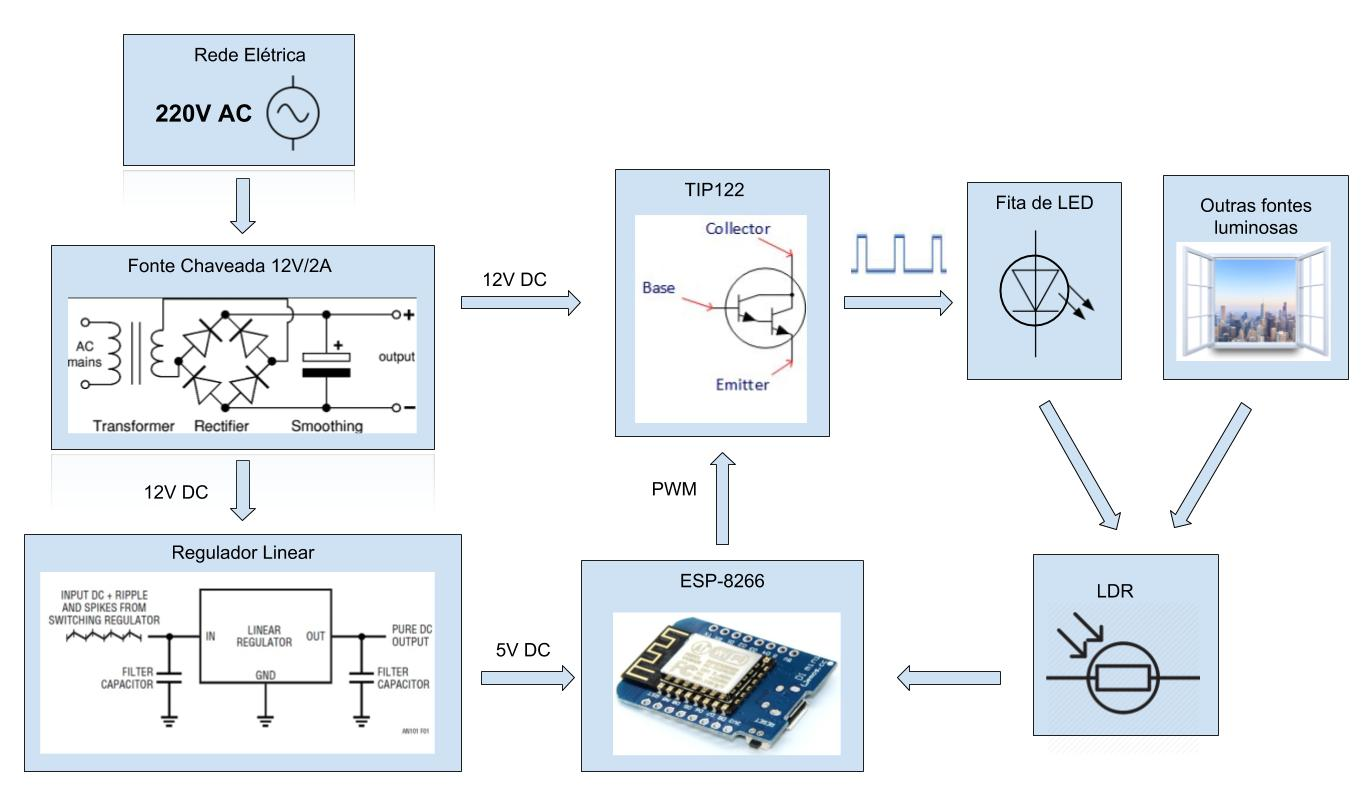
\includegraphics[width=\textwidth]{figuras/esquema_eletrico.jpg}
    \end{center}
    \caption[Esquema geral do projeto da fita de LED MQTT.]{Ilustração do funcionamento do protocolo MQTT com três clientes e o broker trocando mensagens pelo tópico "temperatura".}
    \label{esquema}
\end{figure}

\section{Alimentação}

A fonte de alimentação elétrica do projeto é uma fonte comercial de 12V/1A de padrão comercial “\textit{bivolt}” com plugue P4. Os 12V fornecidos pela fonte serão partilhados pela fonte de iluminação e pelo sistema embarcado. Um regulador baseado no CI AMS1117 será usado para transformar os 12V da fonte em 5V para alimentar o sistema com o microcontrolador. Esse regulador têm sua tensão de saída fixa em 5V e apresenta algumas funcionalidades como limitador interno de corrente e auto-desligamento térmico, e com o arrefecimento adequado ele pode fornecer até 1A que já é mais que o suficiente para o ESP-8266 que consome em torno de 220 mA durante curtos períodos quando está transmitindo via WiFi.

\begin{figure}[ht]
    \begin{center}
    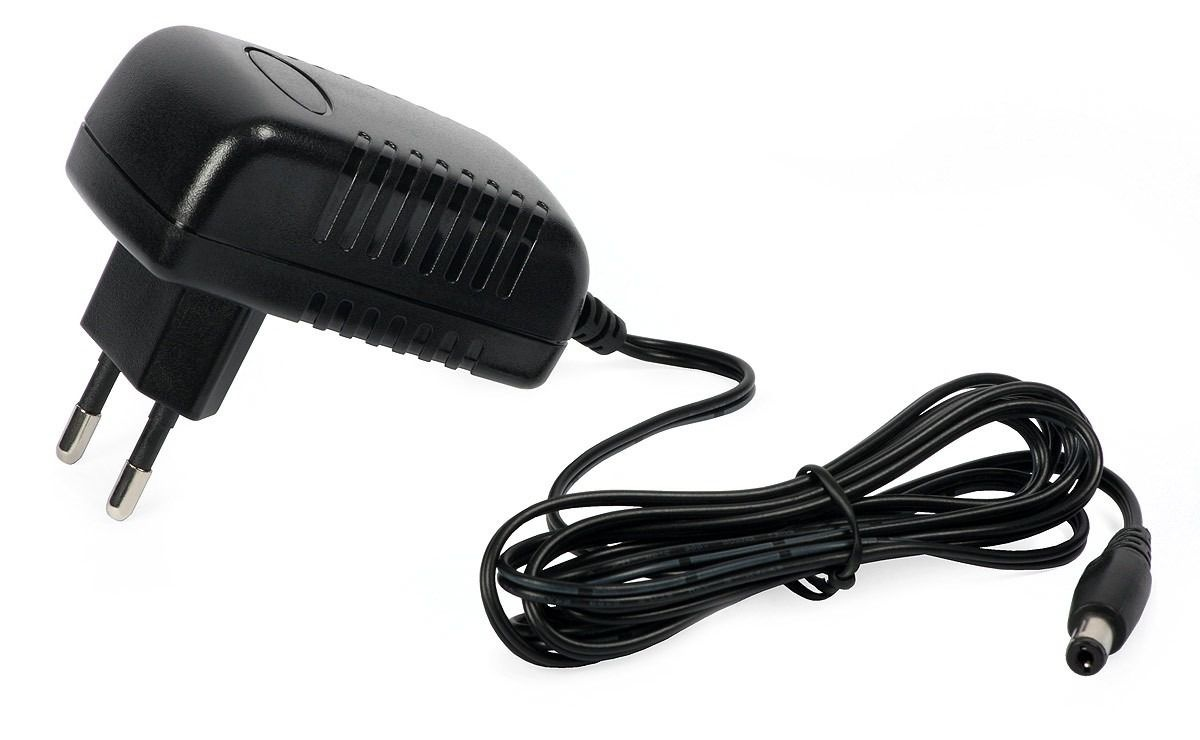
\includegraphics[width=0.5\textwidth]{figuras/fonte.jpg}
    \end{center}
    \caption[Ilustração da fonte chaveada de 12V.]{Ilustração da fonte chaveada de 12V com capacidade de fornecer até 2A.}
    \label{fonte}
\end{figure}

\section{Módulo Microcontrolador}

Como mencionado, o microcontrolador escolhido para o projeto é o ESP-8266 que inclui capacidade de comunicação WiFi. A própria fabricante do CI comercializa alguns módulos que facilitam o desenvolvimento com o ESP-8266 com antenas, LED, memória \textit{flash} e outros periféricos. Um desses módulos, o ESP-12 é usado por diversas empresas para fabricarem seus kits de desenvolvimento com ainda mais facilidades para o desenvolvedor. O kit usado neste projeto é “\textit{Wemos D1 Mini}” que conta com conversor USB-serial, regulador de tensão para transformar os 5V DC provenientes da porta "USB" ou da alimentação externa para os 3.3V DC que o ESP-8266 demanda, oscilador, botão para \textit{reset} e conectores para os pinos de entrada e saída.

\begin{table}
    \centering
    \label{wemos_dados}
    \caption{Especificações do kit \textit{Wemos D1 Mini}}
    \begin{tabular}{ll} 
        \hline
        Kit de desenvolvimento          & Wemos D1 Mini  \\ 
        \hline
        SoC                             & ESP-8266       \\ 
        \hline
        Pinos de I/O digitais           & 11             \\ 
        \hline
        Entradas analógicas             & 1 (3,2V máx)   \\ 
        \hline
        Clock                           & 80 MHz         \\ 
        \hline
        Memória \textit{flash}          & 4 MB           \\
        \hline
    \end{tabular}
\end{table}

O pino de entrada analógica do módulo usado tem uma tensão máxima especificada de 3,2V, apesar de a tensão máxima de entrada do ESP-8266 ser de 1V segundo suas características elétricas \cite{esp}. Isto se deve ao fato de o módulo "\textit{Wemos D1 Mini}" apresentar um divisor de tensão conectado ao pino de entrada analógica do SoC fazendo com que a tensão aplicada a este pino seja mapeada de um intervalo de, 0 a 3,2V no devido pino do módulo, para um intervalo de 0 a 1V no pino do ESP-8266.

\begin{figure}[ht]
    \begin{center}
    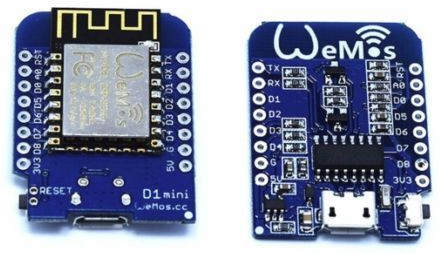
\includegraphics[width=0.4\textwidth]{figuras/wemos.PNG}
    \end{center}
    \caption[Ilustração do módulo \textit{Wemos D1 Mini}.]{Módulo \textit{Wemos D1 Mini} baseado no ESP-8266 visto de cima e de baixo.}
    \label{wemos}
\end{figure}

\section{Sensor de Luminosidade}

O sensor de luminosidade é um "fotoresistor" ou \acf{LDR} cuja resistência, geralmente, diminui com o aumento da intensidade luminosa linearmente. Geralmente são materiais semicondutores de alta resistividade, mas que quando expostos à luz, têm elétrons liberados em sua camada de condução aumentando assim sua condutividade por isso são geralmente chamados de células fotocondutivas. Existem LDRs sensíveis a faixas de radiação ultravioleta, infravermelho e a luz visível, que são os mais comuns.

O LDR usado \cite{ldr} é feito do material semicondutor CdS e apresenta uma curva de resistência em função da intensidade luminosa como mostrada na figura \ref{reta}. Os valores mostrados podem variar um pouco com a temperatura e existe um comportamento transiente quando a luminosidade é variada bruscamente de tempos da ordem de 100ms, o que não se torna relevante para medições menos frequentes que uma repetição por minuto, por exemplo.

\begin{figure}[htp]
    \begin{center}
    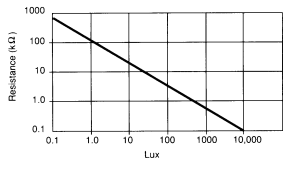
\includegraphics[width=0.4\textwidth]{figuras/reta.PNG}
    \end{center}
    \caption[Gráfico da reisitência \textit{versus} intensidade luminos do LDR.]{Gráfico da reisitência \textit{versus} intensidade luminos do LDR.}
    \label{reta}
\end{figure}

\section{Fita de LED}
A fonte de iluminação é uma fita de LED branca que consiste de elementos de três LEDs e um resistor em série para limitar a corrente, com vários desses elementos ligados em paralelo o que permite que todos os elementos sejam submetidos à mesma tensão e que a fita possa ser cortada em determinados pontos e continue funcionando. A fita de LED adquirida para o projeto tem as especificações listadas na Tabela 3.2.

\begin{figure}[htp]
    \begin{center}
    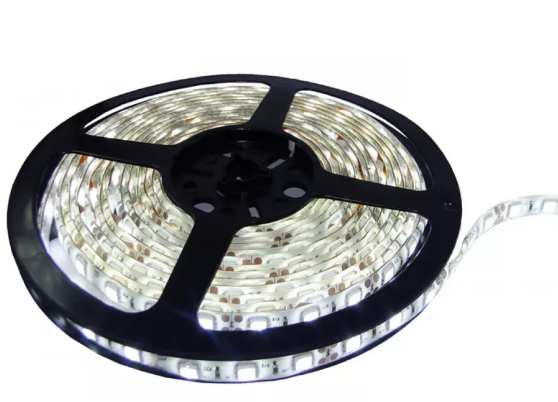
\includegraphics[width=0.3\textwidth]{figuras/fitaled.PNG}
    \end{center}
    \caption[Ilustração da fita de LED branca.]{Ilustração da fita de LED de cor branca fria de 12V.}
    \label{fitaled}
\end{figure}

 

\begin{table}
    \centering
    \label{fitaled_dados}
    \caption{Especificações da fita de LED branca}
    \begin{tabular}{ll} 
        \hline
        Tensão de Operação (V)  & 12            \\ 
        \hline
        Consumo por metro (W/m) & 4.8           \\ 
        \hline
        Comprimento (m)         & 5             \\ 
        \hline
        LEDs por metro          & 60            \\ 
        \hline
        Temperatura da cor (K)  & 6000(frio)    \\
        \hline
    \end{tabular}
\end{table}

O controle da luminosidade será feito por chaveamento da alimentação da fita de LED com \acf{PWM}, técnica que permite controlar digitalmente a potência entregue a atuadores ao determinar a parcela do período em nível lógico alto, de um sinal alternado. O microcontrolador irá chavear um transistor \textit{darlington} “TIP122” \cite{tip122}.

\section{Ferramentas de Desenvolvimento}

\subsection{\textit{Broker} MQTT}

O \textit{broker}, ou servidor, MQTT responsável pelo controle das mensagens intercambiadas na rede será o \textit{broker} da "\textit{Adafruit}" \cite{adafruit}. O serviço oferecido pela \textit{Adafruit} conta com um  \textit{broker} MQTT configurado com níveis de QoS 0 e 1, tópicos especiais como o "\texttt{time/seconds}" que fornece um número de segundos passados desde primeiro de janeiro de 1970 (\textit{Unix Time}) ou o tópico "\texttt{(username)/throttle}" que indica se a limitação de frequência de publicações foi atingida (que na versão grátis do serviço é de 60 vezes por minuto). O seviço da \textit{Adafruit} fornece também uma biblioteca da MQTT própria para \textit{Arduino} que define várias funções de \textit{callback} de subscrições e rotinas de conexão, desconexão e outras.

Uma interface de controle e visualização \textit{web} também é fornecida pela \textit{Adafruit} com possibilidade de implementação de botões, mostradores de valores, gráficos em tempo real, entre outras funcionalidades.

\subsection{Ambiente de Desenvolvimento de \textit{Software}}

O ESP-8266 possui um conjunto de bibliotecas e ferramentas, cujo objetivo é produzir código que, quando compilado, pode ser gravado na memória de programa e executado. Essas ferramentas levam o nome de "SDK" (\textit{Software Development Kit}) e são fornecidas, oficialmente, pela fabricante \textit{Espressif}. Uma comunidade de desenvolvedores do ESP-8266 criou uma estrutura de interfaces e adaptações (\textit{framework}) de código aberto para a SDK oficial para que fosse possível programar com a linguagem "C++" e usar as bibliotecas do \textit{Arduino}.

O desenvolvimento do software foi feito na IDE (\textit{Integrated Development Environment}) "\textit{Visual Studio Code}" da "\textit{Microsoft}" que é essencialmente um editor de texto de código aberto, muitas opções de customização e capacidade de conexão com extensões de terceiros. Uma dessas extensões foi usada, o "PlatformIO", Figura \ref{pio}, que é uma plataforma que conta com compiladores e outras ferramentas de diversos microcontroladores como \textit{Arduino}, ARM, \textit{Atmel} e vários outros. A extensão conta ainda com terminal virtual, monitor de porta serial, ferramentas de depuração de código e suporte à versionamento de código online.

\begin{figure}[ht]
    \begin{center}
    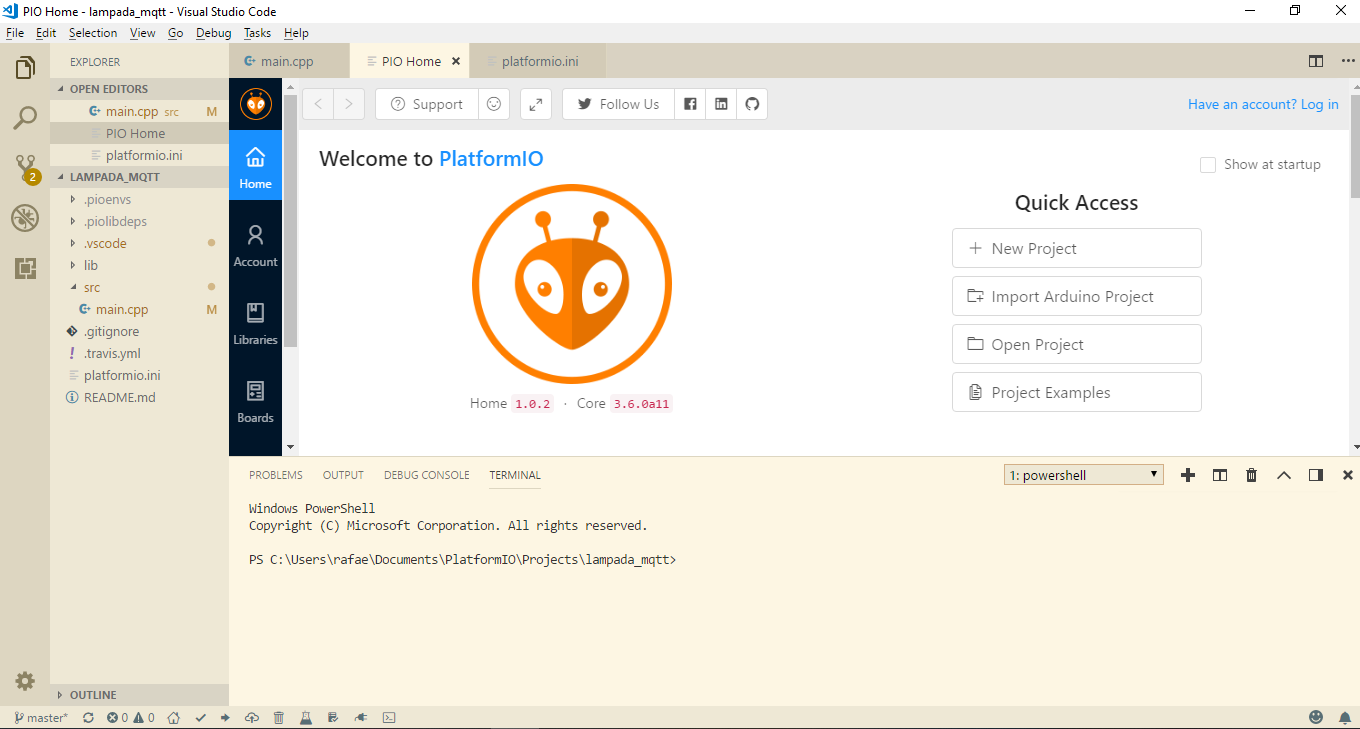
\includegraphics[width=\textwidth]{figuras/pio.PNG}
    \end{center}
    \caption[Ilustração do Visual Studio Code com o PlatformIO.]{Ilustração do ambiente de desenvolvimento "Visual Studio Code" com a extensão "PlatformIO".}
    \label{pio}
\end{figure}

\subsection{Bibliotecas}

Como mencionado, a programação foi feita na linguagem de programação "C++" com algumas bibliotecas de terceiros. A primeira a ser mencionada é a biblioteca do \textit{Arduino} que disponibiliza várias funções e definições que permitem uma grande simplicidade legibilidade do código escrito \cite{arduino}.

Outra biblioteca usada foi "Esp8266WiFi" \cite{espwifi}que disponibiliza várias rotinas relativas a conexão do ESP-8266 como a rede WiFi, reconexão, códigos relativos a camada TCP/IP e outros detalhes importantes para que o uso da internet com o microcontrolador seja possível.

A biblioteca "WiFi \textit{Manager}" \cite{wifimng} foi também usada e permitiu automatizar e generalizar o processo de autenticação do projeto para qualquer rede WiFi por meio da criação de uma página \textit{web} pela qual o usuário pode escolher a rede desejada e informar sua senha para que o ESP-8266 se conecte e salve essas informações em caso de reconexão.

\chapter{Implementação}

O conjunto de sistemas embarcados propostos são integrados em um Controlador Semafórico, dispondo um meio de monitorar, controlar e gerenciar os vários aspectos envolvidos no ambiente urbano, em relação ao trânsito. O controlador semafórico é uma solução que envolve diferentes equipamentos, com objetivos específicos cada, que interligados apresentam um meio de ordenar o fluxo veicular e de pedestres em seu entorno.

Com a utilização de microcontroladores, o planejamento de circuitos eletrônicos e a programação de firmwares dedicados, o controlador semafórico é responsável por realizar o acendimento e monitoramento da sinalização semafórica, sendo suas funções mais relevantes para tal solução: acendimento de grupos focais (lâmpadas de semáforos) veiculares, acendimento de grupos focais para pedestres, detecção de demanda de travessia de pedestres, sinalização de tempo restante de passagem de veículos (display acoplado aos grupos focais, exibindo um contador regressivo).

Cada sistema, individualmente, possui um propósito específico, e foi planejado de modo otimizado, para apresentar confiabilidade, fácil funcionamento e custo reduzido. Os microcontroladores utilizados para alcançar os objetivos foram da família PIC e da família AVR, sendo, especificamente, o PIC16F77, PIC12F675 e AT89S8253. Em cada aplicação, diferentes funcionalidades dos microcontroladores foram utilizadas, dependendo das necessidades apresentadas.


\section{Placa de controle de acendimento semafórico}

\begin{figure}[ht]
    \begin{center}
    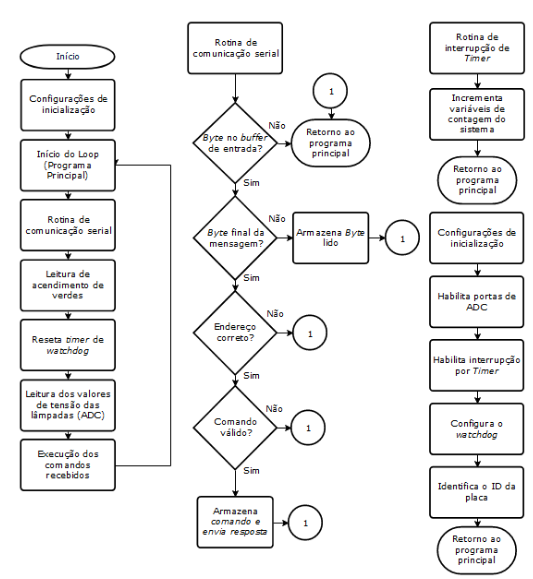
\includegraphics[width=0.8\textwidth]{figuras/fluxo_fase.PNG}
    \end{center}
    \caption[Placa de fase]{Fluxograma de funcionamento do firmware da placa de controle de acendimento.}
    \label{placa_fase}
\end{figure}

A placa de controle de acendimento semafórico tem como função assegurar o funcionamento correto do semáforo, tanto veicular quanto de pedestres, sendo responsável pelo acendimento e monitoramento dos focos, assegurando a sequência correta de cores do semáforo (Verde > Amarelo > Vermelho).
%[http://meusite.mackenzie.br/professor_cucci/ManualSemaforos2014.pdf]. 

O microcontrolador utilizado na placa é um PIC16F77, que possui 40 pinos e capacidade de processamento de 8 bits. Um cristal é utilizado, para gerar uma velocidade de clock de 20 MHz, e cada instrução é realizada a cada 200 ns (4 ciclos do clock). Esse dispositivo é utilizado para chavear a tensão da rede elétrica e monitorar o acendimento semafórico, e enviar as informações para a central do controlador semafórico.

O firmware da placa foi escrito especificamente para o dispositivo utilizado realizar as funções desejadas. A FIGURA X apresenta os processos realizados pelo microcontrolador durante o seu funcionamento. A placa aguarda os comandos vindos da central (CPU) do controlador semafórico para executar o acendimento dos focos. Os comandos são recebidos pela porta serial (USART) do PIC16F77, através de comunicação assíncrona.

O acendimento de cada foco é realizado com a utilização de um optoacoplador, em conjunto com um TRIAC. O optoacoplador é um dispositivo que permite o isolamento de dois circuitos, utilizando luz emitida por um LED para acionar a outra parte do circuito, 
%[Rudolf F. Graf (1999). Modern dictionary of electronics. Newnes. ISBN 0-7506-9866-7.], 
enquanto o TRIAC é um dispositivo que permite a passagem de corrente nas duas direções, a partir de ativação através de um terceiro pino. 
%[M.D. Singh, K.B. Khanchandani, Power Electronics, Second Edition, Tata McGraw-Hill, New Delhi, 2007, pages 148-152]. 
Utilizando esses dois componentes, é possível realizar o controle da tensão da rede elétrica (220 V) utilizando um sinal de 5 V dos pinos de I/O do microcontrolador.

O acendimento de cada foco é dado pelo controle do pino do PIC responsável por cada cor (verde, amarelo, vermelho). Ao executar o comando de acender foco, o pino é colocado em 0 V, ativando assim o optoacoplador, e fazendo passar o neutro, da rede elétrica, para o foco semafórico, resultando em seu acendimento.

\begin{figure}[ht]
    \begin{center}
    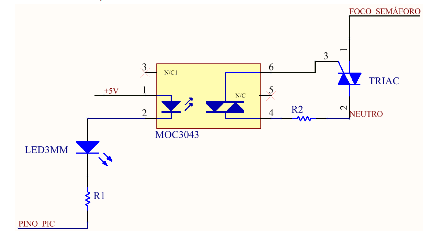
\includegraphics{figuras/moc_triac.PNG}
    \end{center}
    \caption[Acendimento semafórico]{Circuito responsável pelo acendimento semafórico.}
    \label{moc_triac}
\end{figure}

O PIC16F77 possui um conversor A/D com precisão de 8 bits, que é utilizado, no projeto, para realizar a leitura do valor da tensão da carga, que é o foco, quando aceso. O sinal passa por um transformador abaixador e uma ponte retificadora, para ser lido pelo pino do PIC, que resulta em um valor de leitura proporcional à potência da carga utilizada. Esse circuito permite ao sistema ter capacidade de monitorar diversos estados das lâmpadas utilizadas no semáforo, sendo eles subtensão, funcionamento esperado, sobretensão e queima.

\begin{figure}[ht]
    \begin{center}
    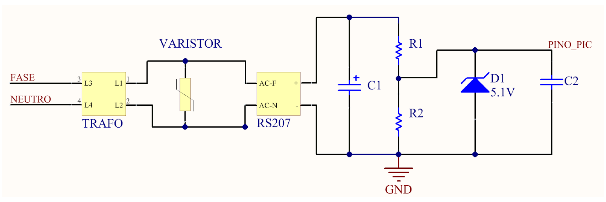
\includegraphics[width=0.5\textwidth]{figuras/trafo.PNG}
    \end{center}
    \caption[Detecção da lâmpada]{Circuito responsável pela leitura do sinal analógico.}
    \label{trafo}
\end{figure}

Outra função da placa é o monitoramento de acendimento dos focos, em que o PIC realiza a leitura de cada foco (verde, amarelo, vermelho) de uma fase e armazena os valores lidos. A leitura é realizada no pino de saída de um optoacoplador, o qual é ativado pela presença de fase e neutro (rede elétrica) na sua entrada. A placa possui um circuito separado para cada foco monitorado, cada um ocupando um pino diferente de I/O do PIC.

\begin{figure}[ht]
    \begin{center}
    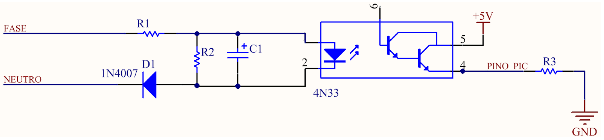
\includegraphics[width=0.5\textwidth]{figuras/4n33.PNG}
    \end{center}
    \caption[Detecção de presença de fase]{Circuito responsável pelo monitoramento de acendimento dos focos.}
    \label{4n33}
\end{figure}

Além das funções já mencionadas, o PIC é configurado para habilitar interrupção por timer. O timer é utilizado como contador para o controle das funções temporizadas do sistema. 

\section{Placa de controle de contagem de tempo semafórico}

\begin{figure}[ht]
    \begin{center}
    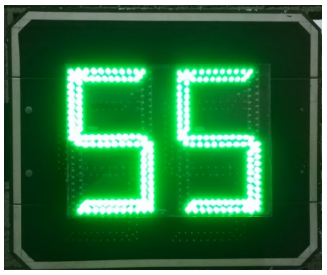
\includegraphics{figuras/cronometro.PNG}
    \end{center}
    \caption[Sistema de cronômetro]{Cronômetro marcador de tempo semafórico.}
    \label{cronometro}
\end{figure}

A placa de controle de contagem de tempo semafórico tem como finalidade realizar a contagem, e mostrar no display, como mostrado na Figura \ref{cronometro}, do tempo de passagem veicular, enquanto o grupo focal estiver aceso no estado verde.

O microcontrolador utilizado é um AVR AT89S8253, que possui 40 pinos e capacidade de processamento de 8 bits. Um cristal é utilizado, para gerar um clock de 12 MHz, e cada instrução é realizada a cada 12 ciclos do clock. O dispositivo é utilizado para realizar as funções de detectar o acendimento do verde no semáforo, contar, e salvar em memória, o tempo de verde e exibir o tempo em um display de 7 segmentos. O fluxo do firmware utilizado nesse microcontrolador pode ser visualizado na Figura \ref{fluxo_cron}.

\begin{figure}[ht]
    \begin{center}
    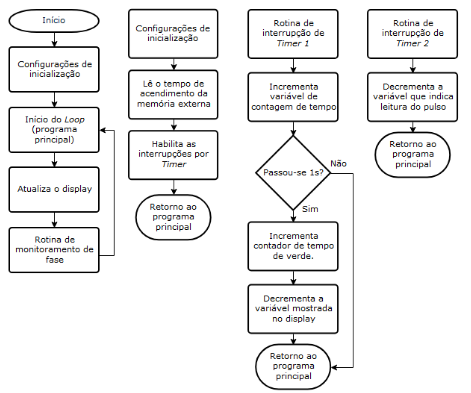
\includegraphics{figuras/fluxo_cron.PNG}
    \end{center}
    \caption[Fluxograma do sistema de cronômetro]{Funcionamento do firmware do sistema de contagem de tempo semafórico.}
    \label{fluxo_cron}
\end{figure}

O equipamento de contagem é instalado acoplado ao foco semafórico e é eletricamente conectado em paralelo com a fase verde do semáforo. Como não existe comunicação entre a placa de cronômetro e o controlador semafórico, o início da contagem do tempo é determinado pela detecção de acendimento do semáforo. Ao detectar a presença da rede elétrica, o microcontrolador busca na memória o valor da contagem de tempo de verde e inicia a contagem regressiva. Caso não exista valor salvo na memória, é carregado um valor padrão.

\begin{figure}[ht]
    \begin{center}
    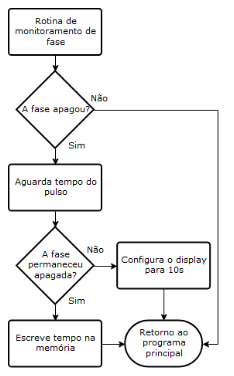
\includegraphics{figuras/fluxo_cron2.PNG}
    \end{center}
    \caption[Fluxograma do monitoramento do cronômetro]{Fluxo da rotina de monitoramento da fase veicular.}
    \label{fluxo_cron2}
\end{figure}

Após iniciar a contagem, o microcontrolador passa a monitorar a fase acesa, de acordo com a rotina demonstrada na FIGURA. O controlador semafórico possui um método para indicar que o tempo de verde está próximo do fim, na forma de um pulso, com duração de 100 ms, durante o qual a alimentação é retirada da placa de contagem. Esse método é importante para assegurar o funcionamento correto do sistema nas determinadas situações:

\begin{itemize}
\item No ciclo inicial, em que o microcontrolador ainda não possui valor de tempo gravado na memória.
\item Após mudanças dos planos, quando o tempo de acendimento passar a ser diferente do tempo armazenado na memória.
\end{itemize}

O pulso é necessário nessas situações, pois são cenários em que ocorre dessincronização entre a placa de contagem e o controlador semafórico, e os displays não exibem o tempo correto. Ao reconhecer o pulso, porém, a placa entra em sincronia com o controlador e exibe o valor correto no mostrador (o pulso indica que faltam 10 s de tempo de verde). Ao apagar o foco verde, o microcontrolador reconhece a ausência de alimentação por mais de 100 ms, e salva na memória o tempo do ciclo de acendimento.
No equipamento são utilizados dois timers distintos para gerar interrupções. O primeiro é utilizado para a contagem do tempo e atualização da variável que é exibida nos displays. O segundo é utilizado para a contagem dos 100 ms para reconhecimento do pulso do controlador.

\section{Placa de detecção de demanda de atuadores externos}

\begin{figure}[ht]
    \begin{center}
    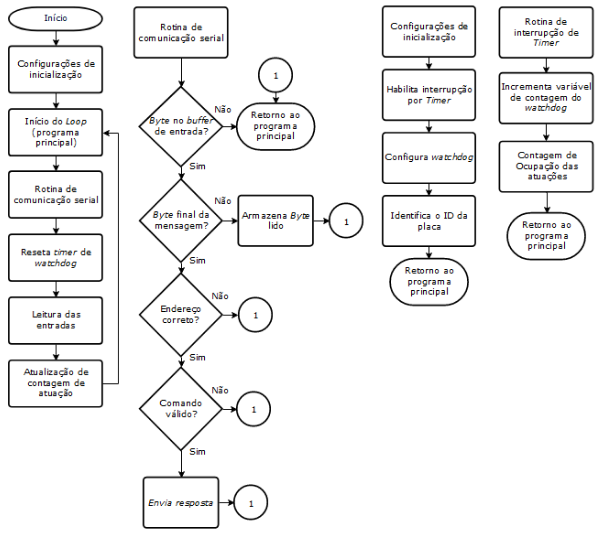
\includegraphics{figuras/fluxo_atdr.PNG}
    \end{center}
    \caption[Fluxograma do atuador]{Fluxo do funcionamento de detecção de demanda.}
    \label{fluxo_atdr}
\end{figure}

A placa de monitoramento de demanda de atuadores externos tem como finalidade acumular as demandas vindas de atuadores externos, ativados por pedestres para realizar a travessia de vias. A placa recebe um sinal, referente às atuações, do equipamento que realiza o registro das demandas, à medida que vão ocorrendo, e utiliza esse sinal para realizar cálculos referentes à quantidade e volume de demandas registradas.

Assim como a placa de controle de acendimento semafórico, o microcontrolador utilizado nessa placa é um PIC16F77, utilizando, também, um cristal de 20 MHz para gerar o clock. As funções necessárias para essa placa são:

\begin{itemize}
\item Comunicação com a CPU
\item Registro de atividades de atuadores externos
\item Cálculo de quantidade de demanda em um determinado intervalo de tempo
\item Cálculo de volume de demandas em um determinado intervalo de tempo
\end{itemize}

O firmware escrito para essa placa segue o fluxo que pode ser visto na Figura \ref{fluxo_atdr}, que apresenta os processos realizados pelo microcontrolador durante seu funcionamento. Para realizar a comunicação com a CPU, é utilizada a porta serial do PIC, através de uma comunicação assíncrona. 

\begin{figure}[ht]
    \begin{center}
    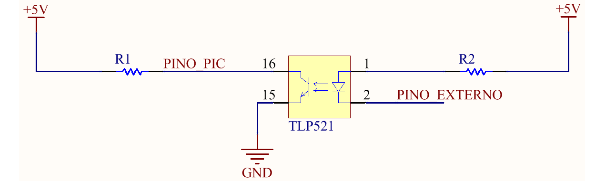
\includegraphics{figuras/atuacao.PNG}
    \end{center}
    \caption[Circuito de atuador]{Circuito responsável pela detecção de atuação.}
    \label{atdr}
\end{figure}

Como pode ser visto na Figura \ref{atdr}, o circuito de monitoramento das demandas possui um optoacoplador, que é ativado quando o equipamento que registra as demandas envia o sinal por meio do pino externo, e o PIC detecta a atuação. Além desses dados, o PIC incrementa uma contagem cada vez que uma demanda é registrada, desse modo armazenando a contagem de atuação para cada detector.

Além da contagem de atuação, outra funcionalidade da placa é o armazenamento do volume das atuações. Para isso, o timer do microcontrolador é utilizado. Durante a rotina de interrupção do timer, o PIC identifica as demandas recebidas e calcula, durante uma janela de tempo (determinada pela CPU), durante que porcentagem desse período as demandas ficaram ativas. Essas informações armazenadas são enviadas para a CPU, por meio da porta serial, quando requisitadas.

\section{Placa de registro de demanda de pedestre}

A interface por aplicação móvel para sistemas 

\section{Integração}

A interface \textit{web} é uma das funcionalidades ofertadas pelo serviço da \textit{Adafruit} e têm \textit{widgets} bem parecidos com os do aplicativo móvel; com uma diferença principal: Há um widget que plota um gráfico temporal dos valores publicados em algum dos tópicos e permite que os dados de qualquer tópico possam ser salvos em um arquivo "csv", formato compatível com os principais editores de planilhas.

\chapter{Integração}

Cada equipamento apresentado nesse trabalho desempenha um papel importante no controle e monitoramento da sinalização semafórica nas vias urbanas. Para que todos os processos ocorram de forma ordenada e sincronizada, é necessário que se realize a integração entre os sistemas com o controlador semafórico. Essa integração pode ser dividida em duas etapas: o controle veicular e o controle de pedestres. Essas duas etapas 

\section{Controle veicular}

O controle veicular é realizado pelas placa de controle de acendimento semafórico e placa de controle de contagem de tempo semafórico. A placa de acendimento é controlada pela CPU do controlador semafórico, e é responsável pelo acendimento dos semáforos. A placa de contagem é instalada 

\section{Controle de pedestres}

\section{Controlador semafórico}
\subsection{Elementos internos}
\subsection{Elementos externos}
\chapter{Considerações finais}

Os microcontroladores são versáteis e capazes de realizar as tarefas propostas neste trabalho, de monitorar e controlar o trânsito em regiões urbanas, de maneira automatizada e integrada, fazendo parte de soluções adotadas, com o intuito de tornar as experiências em locais urbanos seguras e ordenadas.

Foram apresentados diferentes sistemas, cada um com uma finalidade específica, de modo a aumentar a confiabilidade no funcionamento individual. Foi desenvolvida, também, a integração entre todos os equipamentos, para atingir a sincronia entre os processos envolvidos.





%%
%% Parte pós-textual
%%
\backmatter

% Apêndices
% Comente se não houver apêndices
%\appendix

% É aconselhável criar cada apêndice em um arquivo à parte, digamos
% "apendice1.tex", "apendice.tex", ... "apendiceM.tex" e depois
% incluí-los com:
% \include{apendice1}
% \include{apendice2}
% ...
% \include{apendiceM}


% Bibliografia
% É aconselhável utilizar o BibTeX a partir de um arquivo, digamos "biblio.bib".
% Para ajuda na criação do arquivo .bib e utilização do BibTeX, recorra ao
% BibTeXpress em www.cin.ufpe.br/~paguso/bibtexpress
\nocite{*}
\bibliographystyle{ieeetr}
\bibliography{biblio}

% Cólofon
% Inclui uma pequena nota com referência à UFPEThesis
% Comente para omitir
\colophon

%% Fim do documento
\end{document}
